[...]\todo[color=red]{A brief introduction to the chapter.}

\section{The Herschel-ATLAS}
\label{sec:The Herschel-ATLAS}

The \textit{Herschel} Astrophysical Terahertz Large Area Survey (H-ATLAS; \citealt{Eales_2010}) was the largest open-time sub-mm survey carried out with \textit{Herschel}. The survey was observed across five photometric bands using two instruments onboard the \textit{Herschel Space Observatory}: the Photodetector Array Camera (PACS, \citealt{Poglitsch_2010}) at 100 and 160\,\micron, and the Spectral and Photometric Imaging Receiver (SPIRE, \citealt{Griffin_2010}) at 250, 350 and 500\,\micron. Compared to the first SMGs detected using SCUBA at 850\,\micron (\citealt{Smail_1997}; \citealt{Barger_1998}; \citealt{Hughes_1998}), the PACS and SPIRE wavebands span the peak of the infrared spectrum for low redshift (z < 1) galaxies. Their intrinsic brightness at the SPIRE wavelengths makes their detection in the thousands more achievable. The main scientific goal of the survey was to estimate the dust masses and dust obscured star formation rates for thousands of nearby galaxies over a large area of sky. While the intention was for a shallow survey, the surprising sensitivity of \textit{Herschel} and the negative k-correction observed at the operating wavelengths of the SPIRE instrument (\citealt{Blain_1993}) means that many sources were observed at higher redshifts, with a median of z $\sim$ 1. The catalogues of the survey, as detailed below, includes sources with redshifts up to $\sim$ 6 (\citealt{Amblard_2010}; \citealt{Lapi_2011}; \citealt{Fudamoto_2017}; \citealt{Zavala_2018}).

The complete survey covers $\sim$\,660\,$\deg^2$, split into three regions located to avoid emission from Galactic dust and to utilize complimentary spectroscopic surveys including the Sloan Digital Sky Survey (SDSS, \citealt{York_2000}), the 2df Galaxy Redshift Survey (2dfGRS, \citealt{Colless_2001}) and the Galaxy and Mass Assembly (GAMA, \citealt{Driver_2009}). The North Galactic Pole (NGP) region covers $\sim$\,180\,$\deg^2$ of the northern sky, centered at R.A 13$^{h}$18$^{m}$ and declination +29$^{\circ}$13' (J2000); three equatorial fields, located at approximately R.A 9$^{h}$, 12$^{h}$ and 15$^{h}$ coinciding with the GAMA survey (henceforth named GAMA9, GAMA12 and GAMA15 fields), each with an area of approximately 54\,$\deg^2$, and the South Galactic Pole (SGP) region, centered at R.A 0$^{h}$6$^{m}$ and declination -32$^{\circ}$44' (J2000) with an area of $\sim$ 318\,$\deg^2$. 

\subsection{Detecting Submillimeter Sources on Herschel Images}
\label{sec:Detecting Submillimeter Sources on Herschel Images}

Due to [...]\todo[color=orange]{continuation:} sub-mm images suffer from two types of noise; instrumental noise [...]\todo[color=orange]{continuation:} and confusion noise which is highly correlated between pixels, most of its contribution coming from the blending together of faint sources. Source confusion is of particular importance to sub-mm surveys [...]\todo[color=orange]{continuation:}. The result of combining instrumental noise with confusion noise is that almost all sources in the Herschel images are unresolved and the optimum filter for detecting these unresolved sources is no longer the point spread function (PSF). Consider a \textit{Herschel} map in which there is only one source of noise: an image with instrumental noise but no confusion noise (i.e. there is only one point source and no fainter, confusing sources), the optimal detection of this source is obtained by convolving the image with the PSF of the instrument. On the other hand, a map with no instrumental noise, but many confused point sources would be optimally detected with its best signal to noise ratio (SNR) by taking the Fourier transform of the image, dividing by the Fourier transform of the PSF and taking the inverse Fourier transform to obtain a perfect deconvolution of the original map (\citealt{Valiante_2016}). For images that have a variable ratio of instrumental to confusion noise like the \textit{Herschel} images of H-ATLAS, \citealt{Chapin_2011} showed that a convolving function or "matched filter" can be calculated to provide the maximum SNR for an unresolved source.

To detect H-ATLAS sources from the 250\,\micron maps using a matched filter (the 250\,\micron band is the most sensitive of the SPIRE bands and given the lower sensitivity of the PACS instrument, all sources detected on the PACS images would also be detected on the SPIRE 250\,\micron image), \citealt{Maddox_2020} developed a source detection algorithm called the Multi-band Algorithm for Source Detection and eXtraction (MADX). The MADX algorithm works in the following way. Firstly, Galactic dust emission is removed from the images using \texttt{Nebuliser}. Next, the images are convolved with the matched filter [...]\todo[color=yellow]{continuation: description of matched filters}. The variance map is created by convolving the map of variance in instrumental noise with the matched filter and adding the confusion noise. It is from this map that the SNR of a detected source is determined. The same process is repeated with the 350 and 500\,\micron maps and interpolated to the same pixel scale as the 250\,\micron maps. The detection map used to extract sources is then generated from a weighted sum of the three SPIRE maps, however, due to the smaller PSF at 250\,\micron which leads to more accurate positions and the increased number of sources when using the 250\,\micron maps, zero weighting is given to the 350 and 500\,\micron images. This has the effect of making the detection map the same as the 250\micron map.

Sources are identified by peak values > 2.5$\sigma$ in the filtered detection map. Their positions are estimated by fitting a Gaussian to the nearest pixels surrounding the location of the peak. The source is extracted in the other \textit{Herschel} wavebands at the 250\,\micron position. Due to the high levels of confusion and high source density on the SPIRE maps, the flux density estimates in each band can be biased by blending with other sources. The MADX algorithm negates some of this problem by ordering the sources by their flux density estimates and iteratively fitting and removing a point source from the position of each source, starting with the brightest. The new estimates of the flux densities are then not influenced by contamination from brighter sources.

The catalogue of point sources provided by H-ATLAS come from the extraction of point sources using MADX applied to the SPIRE images of the NGP, SGP and GAMA fields. The final sources list is reduced to those sources with SNR > 4 in any of the SPIRE bands. While the detection method suggests that we may miss sources that are faint at 250\,\micron but bright at 350 or 500\,\micron, due to the weighting of the three images, cataloguing all sources with SNR > 4 in any of the SPIRE bands means that the catalogues are reasonably complete in all bands. The completeness of the sub-mm catalogues as a function of the measured flux density of a source as estimated by \citealt{Valiante_2016} is illustrated in Figure \ref{fig:submm_completeness}.

\begin{figure}
	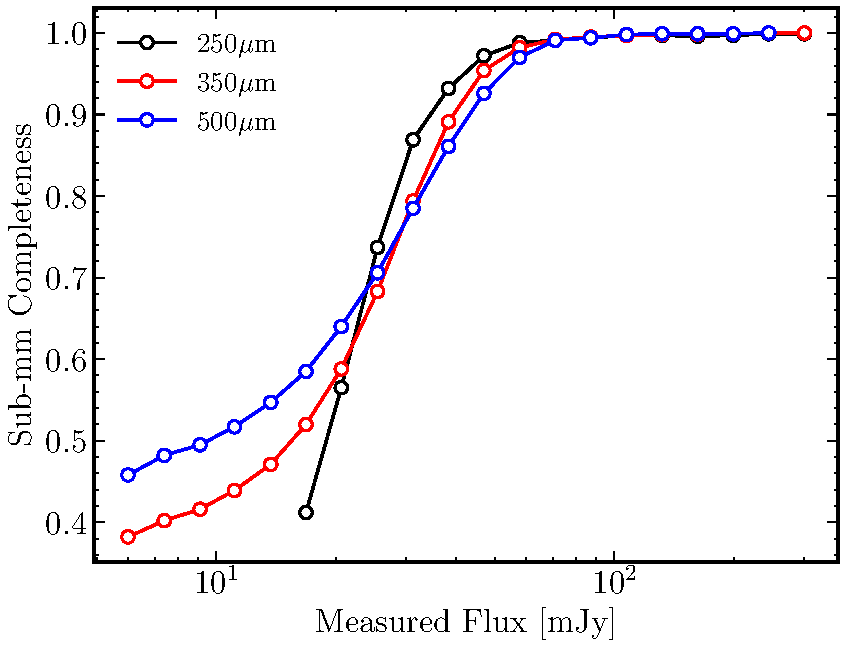
\includegraphics[width=\columnwidth]{Figures/submm_completeness.pdf}
	\caption{The completeness of the H-ATLAS Data Release I catalogues of sub-mm sources, as a function of the measured flux density at 250\,\micron (black) 350\,\micron (red) and 500\,\micron (blue). This figure is replotted from Figure 21 in \citealt{Valiante_2016}.}
	\label{fig:submm_completeness}
\end{figure}

\subsection{Data Releases of the H-ATLAS}
\label{sec:Data Releases of the H-ATLAS}

The first public data release (DR1) of H-ATLAS covered the three equatorial GAMA fields, which span approximately 25\% of the total survey area. These fields benefit from multiwavelength coverage from GAMA, SDSS, 2dF, the Galaxy Evolution Explorer (GALEX, \citealt{Martin_2005}), the UKIRT Infrared Deep Sky Survey -- Large Area Survey (UKIDSS-LAS, \citealt{Lawrence_2007}), the Wide-field Infrared Survery Explorer (WISE, \citealt{Wright_2010}), the VISTA Kilo-degree Infrared Galaxy survey (VIKING, \citealt{Edge_2013}) and the Kilo-Degree Survey (KiDS, \citealt{deJong_2013}). 

Sources are provided with DR1 if they are detected above the 2.5$\sigma$ detection limit on the 250\,\micron map and have measured flux densities greater than the 4$\sigma$ flux density limits in one of the three SPIRE bands (29.6\,mJy, 37.6\,mJy or 40.8mJy at 250, 350 and 500\,\micron). Across the three fields there are a total of 113,995, 46,209 and 11,011 sources detected at > 4$\sigma$ at 250, 350 and 500\,\micron as well as detections for 4,650 and 5,685 sources at > 3$\sigma$ at 100 and 160\,\micron (\citealt{Valiante_2016}). Following the release of the sub-mm sources detected in the GAMA fields, \citealt{Bourne_2016} used the Likelihood Ratio (LR, \citealt{Sutherland_1992}; \citealt{Ciliegi_2003}) method (Section \ref{sec:The Likelihood Ratio Method}) to identify potential optical counterparts to the 113,995 sources with SNR$_{250}$ > 4 from SDSS. Sources with SNR$_{250}$ < 4 that were detected by their 350 or 500\,\micron flux densities were omitted from the matching since these sources have sub-mm colours suggesting a high redshift, and are the most likely sources to be misidentified by SDSS due to the increased probability of chance alignments or gravitational lensing along the line of sight (\citealt{Negrello_2010}; \citealt{Pearson_2013}; \citealt{Bourne_2014}). \citealt{Bourne_2016} found optical counterparts within 10" of 44,385 (39\%) sources with an estimated probability of being the true ID > 80\% (the probability of an optical or near-infrared object being the true counterpart to a sub-mm source is defined as the reliability, R, and is derived in Section \ref{sec:The Likelihood Ratio Method}).

The second public data release (DR2) covered the NGP and SGP, two large fields that together form $\sim$\,75\% of the total survey area. The NGP was covered in the optical by the SDSS and in the near-infrared by UKIDSS-LAS. Moreover, a small area of 25.93\,$\deg^2$ within the NGP was also observed by a deeper K-band survey by the H-ATLAS team using UKIRT (limiting magnitude of K < 19.40 compared to K < 18.69 for UKIDSS-LAS). The SGP is the largest field (approximately half the survey area of H-ATLAS) and was covered by the 2dF spectroscopic survey, KiDS in four optical bands ($u$, $g$, $r$ and $i$) and VIKING in five near-infrared bands ($Z$, $Y$, $J$, $H$ and $K_s$).

Given that sub-mm sources are only extracted from areas of the \textit{Herschel} maps that have at least two obsersations from the SPIRE instrument, the DR2 catalogues includes sources from the map area reduced by the masking of single \textit{Herschel} scans. The mask reduces the area covered by the NGP point source catalogue to 177.1\,$\deg^2$ and the SGP to 303.4\,$\deg^2$. As with DR1, sources are included if they are detected on the 250\,\micron map above the 2.5$\sigma$ detection limit by the MADX algorithm and surpass at least one of the 4$\sigma$ flux density limits at the SPIRE wavelengths. The catalogues contain 118,980 sources for the NGP field (112,069, 48,876 and 10,368 detected at > 4$\sigma$ at 250, 350 and 500\,\micron and 5,036 and 7,046 at > 3$\sigma$ at 100 and 160\,\micron respectively) and 193,527 sources for the SGP field (182,282, 74,096 and 16,084 at 250, 350 and 500\,\micron and 8,598 and 11,894 at 100 and 160\,\micron). \citealt{Furlanetto_2018} applied the Likelihood Ratio method to all counterparts within 10" of the 250\,\micron sources of the NGP using both the shallower optical and near-infrared catalogue of SDSS and UKIDSS-LAS, and the deeper K-band survey. Of the 112,155 SPIRE sources with SNR$_{250}$ > 4, 77,521 (69.1\%) had at least one shallow optical counterpart and 42,429 (37.8\%) of these were matched with R > 0.8. In the smaller area observed with WFCAM, \citealt{Furlanetto_2018} identified 32,041 possible deep near-IR counterparts to 17,247 sources. 10,668 (61.9\%) of these sources were matched with an equally high reliability. While this analysis suggests that the inclusion of deeper K-band data drastically increases the fraction of sources matched to their corresponding optical or near-IR counterpart, [...]\todo[color=yellow]{continuation: we must consider their differences and think about Q}.

In the SGP a preliminary counterpart analysis was conducted using the Two Micron All Sky Survey (2MASS, \citealt{Skrutskie_2006}), but no formal LR analysis had yet been applied. A nearest neighbour match within 5" of a 2MASS galaxy gives identifications for 3,444 \textit{Herschel} sources. In the following section we detail the Likelihood Ratio method and apply it to the 250\,\micron sources detected by \textit{Herschel} in the SGP.

\subsection{Identifying Optical and Near-IR Counterparts to Herschel Sources}
\label{sec:Identifying Optical and Near-IR Counterparts to Herschel Sources}

When identifying multiwavelength counterparts across surveys the simplest choice to use the nearest neighbour within a fixed search radius of one of the sources. For surveys conducted at similar wavelengths with a similar resolution and sensitivity this is a suitable approach. However, when matching far-IR/sub-mm surveys to optical/IR data, the poor angular resolution of long wavelength instruments such as SPIRE (the FWHM of 250\,\micron detections with SPIRE is $\sim$ 18"), which cause large positional uncertainties, force us to increase the search radius around the sub-mm source. This effect, coupled with the intrinsic faintness of optical/near-IR counterparts due to dust obscuration, the relatively flat redshift distribution of sub-mm sources due to the k-correction and the high surface density of objects in optical/IR surveys, means that [...]\todo[color=yellow]{continuation: identification is not easy, Casey reference?} and it is common for there to be multiple possible counterparts within the search radius from a single sub-mm source.

Previously for sub-mm surveys it would be more practical to first match sources with radio or mid-IR sources and then use pre-existing matched catalogues to obtain multiwavelength data (e.g. \citealt{Ivison_2007}; \citealt{Dye_2009}; \citealt{Biggs_2011}, see also Section [...]\todo[color=green]{add reference for the final chapter}). However, presently this is not suitable for large surveys such as H-ATLAS as current radio telescopes do not provide the area and depth required to match with more than a small fraction of sub-mm sources. While current and future radio surveys from facilities such as the Square Kilometre Array (SKA), the Low Frequency Array (LOFAR) and MeerKAT will increase the radio coverage of the H-ATLAS fields, currently a statitstical identification method is still the preferred way of deciding which objects are associated and which are unrelated foreground/background objects to large samples of sub-mm sources.

\subsection{The Likelihood Ratio Method}
\label{sec:The Likelihood Ratio Method}

The Likelihood Ratio method assigns a probability (reliability) to all potential matches surrounding low resolution sources to distinguish between likely counterparts and chance alignments and has been used many times to identify counterparts to \textit{Herschel} sources. The LR method was used by \citealt{Smith_2011} to identify SDSS counterparts in the Science Demonstration Phase (SDP) catalogue (a preliminary data release for H-ATLAS, overlapping with the GAMA9 field), by \citealt{Kim_2012} to identify Spitzer-IRAC counterparts also in the SDP data, by \citealt{Fleuren_2012} for VIKING IDs in the Phase 1 catalogue of the GAMA9 field, and as mentioned earlier, by \citealt{Bourne_2016} and \citealt{Furlanetto_2018} to find optical and near-IR counterparts in the GAMA fields and NGP field respectively.

The likelihood, $L$, of a counterpart being the true identification to a \textit{Herschel} source is given by the ratio between the probability that an object observed at a given radius from the source, $r$, with an optical or near-IR magnitude, $m$, is the true identifcation and the probability of observing an unassociated object with the same $r$ and $m$. On the assumption that the distance from the source and the optical/near-IR magnitude are independent on their influence on the probability of being a true counterpart, we find that:

\begin{equation}
\label{eq:likelihood_ratio}
    L = \frac{P(\textrm{ID}, r, m)}{P(\textrm{unassociated}, r, m)} = \frac{P(\textrm{ID}, r) P(\textrm{ID}, m)}{P(\textrm{unassociated}, r, m)}
\end{equation}

Each term in the above equation can be defined in the following way: $f(r) \coloneqq P(\textrm{ID}, r)$, $q(m) \coloneqq P(\textrm{ID}, m)$ and $n(m) \coloneqq P(\textrm{unassociated}, r, m)$, where $f(r)$ represent the radial probability distribution function of positional errors between the source and counterpart, $q(m)$ represents the magnitude probability distribution of true counterparts and $n(m)$ is the magnitude distribution of background objects from the input survey. By using Baye's theorem and the theorem of total probability, we can define the probability that a counterpart is the true ID given it has $r$ and $m$ as:

\begin{equation}
\label{eq:reliability_one_counterpart}
    R \coloneqq P(\textrm{ID}| r, m) = \frac{L}{L+1}.
\end{equation}
\todo[color=green]{Requires a derivation}

Equation \ref{eq:reliability_one_counterpart} assumes that there is only a single candidate with a likelihood $L$. For a source with multiple possible candidates, the reliability $R_j$ of the $j^{th}$ candidate is given by:

\begin{equation}
    \label{eq:reliability_multiple_counterparts}
        R_j = \frac{L_j}{\sum_i L_i + (1-Q)},
\end{equation}

where $i$ represents the $i^{th}$ counterpart found within the search radius. The $Q$ parameter represents the fraction of all true counterparts that are brighter than the limiting magnitude of the input survey and can therefore be observed. This means that the (1 - $Q$) term represents the probability that the counterpart is not observed and accounts for the fact that not all counterparts will be detected in the optical/near-IR survey. The value of $Q$ depends on the depth of the survey and the choice of passband used. In the following sections I shall outline the methods used to estimate the functions $f(r)$, $q(m)$ and $n(m)$ and to estimate $Q$ to calculate the likelihood ratios and reliabilities of near-IR counterparts observed on the VIKING images surrounding the 250\,\micron positions of \textit{Herschel} sources in the SGP.

\section{Applying the LR Method to VIKING Galaxies in the SGP}
\subsection{VISTA VIKING Counterparts}

The Visible and Infrared Survey Telescope for Astronomy (VISTA) is a 4\,m wide field telescope located at the ESO Paranal Observatory in Chile. The telescope has five near-IR broad band filters, $Z$, $Y$, $J$, $H$ and $K_s$, that have central wavelengths between 0.88 and 2.15\,\micron (\citealt{Emerson_2010}). The VIKING survey was a public survey with VISTA, covering approximately 1,500\,$\deg^{2}$ of sky, including an overlap of more than 360\,$\deg^{2}$ with the H-ATLAS survey in the GAMA and SGP fields, to a 5\,$\sigma$ depth of 23.1, 22.3, 22.1, 21.5 and 21.2 (AB) in the above five filters.

We take as our object catalogue all objects observed in the fourth data release of VIKING within 15" of the 250\,\micron position of each \textit{Herschel} source. The counterpart matching in the GAMA9 field by \citealt{Fleuren_2012}, recovered 51\% of all 250\,\micron sources with a reliable (R > 0.8) VIKING counterpart. Compared to the optical r-band of the SDSS as used in \citealt{Bourne_2016} and \citealt{Furlanetto_2018} which have typical returns of $\sim$ 35 -- 40\% due to the limiting magnitude of SDSS, we expect the SGP to have reliable identifications for approximately half of all SGP sources. The SGP fields contains 193,527 sources detected at greater than 4\,$\sigma$ significance, suggesting that we might expect to match $\sim$ 100,000 \textit{Herschel} sources with a near-IR counterpart with a high probability.

However, a significant number of sources in the VIKING survey are stars that would be erroneously matched to H-ATLAS. The sub-mm emission from stars is most likely from debris discs or dust in outflows. As there is large variation in the mass and temperature of debris discs for stars of a given spectral type (\citealt{Hillenbrand_2008}), and \textit{Herschel} is only sensitive to the brightest of these discs (\citealt{Thompson_2010}), there is much scatter in the sub-mm properties of \textit{Herschel} detected stars which would result in poor statistics of dusty stars when calculating the likelihood of counterparts. For this reason, I use an adapted method of \citealt{Baldry_2010} to separate stars and galaxies in the VIKING SGP catalogue and apply the LR method separately for the two classes.

The method of \citealt{Baldry_2010} uses near-IR $J$ and $K_s$ and optical $g$ and $i$ bands to define a line of separation between stars and galaxies in $J - K_s$, $g-i$ colour-colour space, and is used in \citealt{Bourne_2016} and \citealt{Furlanetto_2018} to separate stellar and extragalactic objects in SDSS. Without coverage from SDSS in the SGP, I use the fourth data release of KiDS to identify optical $g$ and $i$ bands for [...]\todo[color=green]{Look up value} of our VIKING sources. A nearest neighbour search to a maximimum of 0.5" from the 250\,\micron position of each source was used.

First, I classify as stellar any object in our catalogue with \texttt{pStar} > 0.95, an estimate of the probability that the source is a star, based on a shape parameter provided as part of the VIKING data release. This immediately classifies 51,508 objects as stars. Next I consider the $J - K_s$, $g-i$ colour-colour space and define a stellar locus by converting the locus in \citealt{Baldry_2010} to the Vega system assuming $J_{\textrm{Vega}}$ = $J_{\textrm{AB}}$ - 0.91 and $K_{s,\textrm{Vega}}$ = $K_{s,\textrm{AB}}$ - 1.85:

\begin{equation}
    f_{\textrm{locus}} = 
    \begin{cases*}
        0.228 & $g-i$ < 0.3 \\
        0.05 + 0.615(g-i) - 0.13(g-i)^2 & 0.3 $\leq$ $g-i$ < 2.3 \\
        0.7768 & $g-i$ $\geq$ 2.3.
    \end{cases*}
\label{eq:stellar_locus}
\end{equation}

I define a line of separation between stars and galaxies as being +0.2 offset in $J - K_s$ from the stellar locus. The distribution of sources, stellar locus and separation line are illustrated in Figure \ref{fig:star_galaxy_classification}. This classifies a further 411,463 sources that have KiDS identifications (299,525 extragalactic and 111,938 stellar). The remaining objects do not have matches in KiDS and thus do not have $g$ and $i$-band magnitudes. However, based on the separation line defined above, it can be seen that those objects with $J - K_s$ < 0.42 will always fall below the separation line regardless of their optical colour, and similarly, any object with  $J - K_s$ > 0.98 will always lie above the line. The cross contamination of stars above the line and galaxies below the line is small, so I next define all remaining sources using the above single flux cuts. This classifies a further 102,540 sources (102,265 as galaxies and 275 as stars). Finally, I return to the \texttt{pStar} parameter and relax the criteria to those objects with \texttt{pStar} > 0.7; all other objects are classified as galaxies. This method leads to the identifcation of 793,331 (78.9\%) extragalactic sources and 212,028 (21.1\%) stars.

\begin{figure}
	\includegraphics[width=\columnwidth]{Figures/star_galaxy_classification.pdf}
	\caption{The $J - K_s$, $g-i$ colour-colour diagram of VIKING objects with KiDS identifications in the SGP. The stellar locus defined by Equation \ref{eq:stellar_locus} is illustrated as the blue line, while the separation between stars and galaxies, defined as +0.2 offset from the stellar locus, is shown as a dashed blue line. Extragalactic and stellar sources identified from our classification are shown as grey and red points respectively.}
	\label{fig:star_galaxy_classification}
\end{figure}

\subsection{Distribution of True Counterparts, q(m)}
\label{sec:true_counterparts_distribution}

To estimate the reliability of each VIKING source being the true ID to a \textit{Herschel} source, I determine the probability distribution of true counterparts as a function of $K_s$-band magnitude, $q(m)$, using the method described in \citealt{Ciliegi_2003}. First, a magnitude distribution of all objects found in the VIKING images within 15" of a \textit{Herschel} source is generated separately for stars and galaxies, which we shall denote as $n'_{\textrm{total}}(m)$. Here I have set prime notation to reference raw counts, while no prime notation is reserved for counts that have been normalized by the total area searched on the VIKING images. The excess of sources above the background level in regions surrounding the 250\,\micron sources is an estimate for the number density of true VIKING associations and is estimated by subtracting the magnitude distribution for the whole VIKING survey from $n'_{\textrm{total}}(m)$. A set of 844,715 random positions were located on the SGP map and used to search for objects on the VIKING images to within 15". A total of 2,917,214 objects were found and form our $n'_{\textrm{background}}(m)$ distribution. The excess of "real" counterparts thus has a magnitude distribution that may be expected to follow

\begin{equation}
    n'_{\textrm{real}}(m) = n'_{\textrm{total}}(m) - n'_{\textrm{background}}(m) \frac{N_{\textrm{250\,\micron}}}{N_{\textrm{background}}},
\end{equation}

where the distribution has been scaled to the search area by $N_{\textrm{250\,\micron}}$ and $N_{\textrm{background}}$, the number of 250\,\micron positions and the number of randomly located positions respectively.

I then derive the $q(m)$ distribution by normalizing $n_{\textrm{real}}(m)$ and scaling by the fraction of all true counterparts that would be visible on the VIKING images, $Q$. This ensures that the integral of $q(m)$ over all magnitudes up to the limiting magnitude of the VIKING survey is equal to the probability that the sources is detected, i.e. $\int^{m_{\textrm{lim}}} q(m)dm = Q$. This normalization can be written as:

\begin{equation}
\label{eq:true_counterparts_distribution}
    q(m) = \frac{n'_{\textrm{real}}(m)}{\sum_{m_i}n'_{\textrm{real}}(m_i)}\times Q,
\end{equation}

where we have summed over the magnitude bins, $m_i$. The magnitude distribution of "true" counterparts to the 250\,\micron SGP sources is illustrated in the middle panel of Figure \ref{fig:true_counterparts_distribution} and shows the difference between the two distributions for extragalactic and stellar sources, requiring us to implement the LR method separately for the two classes. I also show in Figure \ref{fig:true_counterparts_distribution} the magnitude distributions of $n_{\textrm{total}}$ and $n_{\textrm{background}}$ and the distributions $q(m)/n(m)$ (here $n(m)$ references the area-normalized background distribution of sources, as used in Equation \ref{eq:likelihood_ratio} to calculate the likelihood values). The calculation of the likelihood value for each VIKING source thus depends on an estimate for the fraction of true IDs that are observed on the VIKING images, $Q$, which I detail in the following section.

\begin{figure}
    \centering
	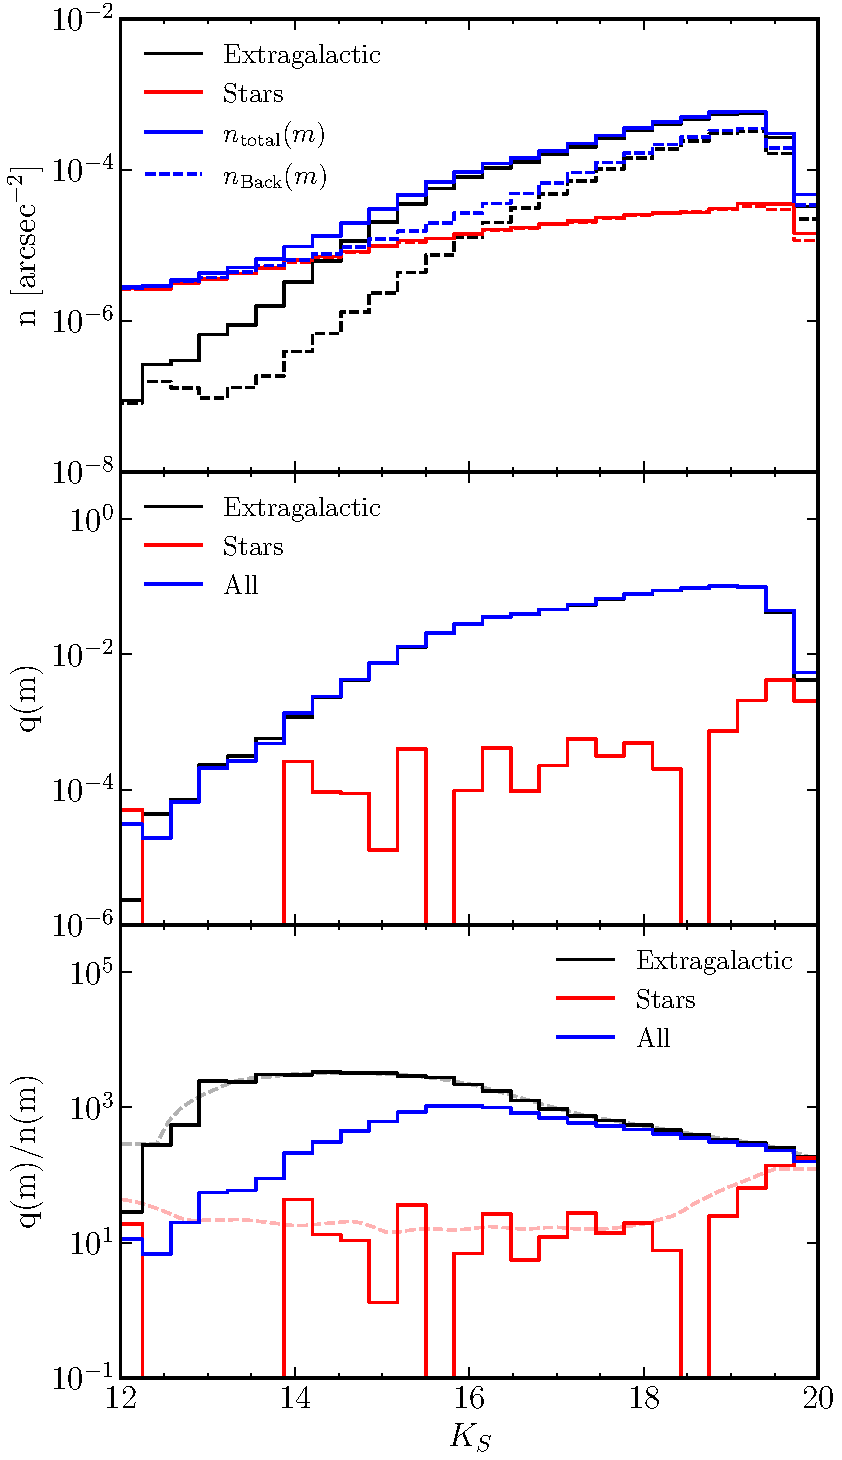
\includegraphics[height=0.75\textheight]{Figures/true_counterparts_distribution.pdf}
	\caption{Top panel: The $K_s$-band magnitude distributions of objects located within 15" of 250\,\micron \textit{Herschel} positions (blue solid line) and random positions (blue dashed line), also separated by extragalactic (black lines) and stellar (red lines) identifications. Middle panel: The $K_s$-band magnitude distribution of "true" counterparts accounting for the excess of VIKING sources observed near \textit{Herschel} sources. Bottom panel: The ratio between the "true" counterparts distribution (middle panel) and the background distribution of sources, as used in the calculation of likelihoods; Equation \ref{eq:likelihood_ratio}. The dashed lines represent smoothed fits to $q(m)/n(m)$ to provide a continuous function at all magnitudes. The colour convention of the middle and bottom panels are the same as the top panel.}
	\label{fig:true_counterparts_distribution}
\end{figure}

\subsection{Estimating Q}

I predict the probability of finding a genuine counterpart in the VIKING images above the limiting magnitude using the method described in \citealt{Fleuren_2012}. While some methods estimate $Q$ directly by totaling the $n_{\textrm{real}}(m)$ distribution and dividing by the number of SPIRE sources, this leads to a systematic overestimate due to the possibility of clustering of galaxies or multiple counterparts to the sub-mm source due to source blending. An alternative method by \citealt{Fleuren_2012} calculates an estimate of 1-$Q_0$, the probability of not observing a VIKING counterpart, by counting the number of sub-mm sources without VIKING associations within a search radius, $r$. These sources will be given the name \textit{blanks}, and has a dependency on search radius, $B(r)$.

Blank sources may be observed in one of several scenarios. The most likely reason (given the limiting depth of VIKING compared to \textit{Herschel}, see Figure [...]\todo[color=orange]{If I include a plot that compares the depth of the surveys against Herschel limits, add reference here.}) is that the real source is fainter than the VIKING $K_s$-band limit. However, a blank may also be observed if the counterpart lies outside the search radius or if the sub-mm source is a spurious SPIRE detection.

While we may observe a sub-mm source with a possible VIKING candidate, we may not definitively say that a source is not a blank as we may encounter chance alignments with VIKING sources close to the same line of sight. Thus, to estimate the true number of blanks, we are reminded that the number of blanks we observe must also account for those that are spuriously identified as not blank. In other words, the number of observed blanks is the number of true blanks minus the number of true blanks that have random VIKING interlopers. If we define the number of observed blanks as $B_{\textrm{obs}}$, the number of true blanks as $B_{\textrm{t}}$ and the number of random interlopers as $N_{\textrm{rand}}$, then

\begin{equation}
    B_{\textrm{obs}} = B_{\textrm{t}} - N_{\textrm{rand}} = B_{\textrm{t}} - B_{\textrm{t}} \times f_{\textrm{rand}},
\end{equation}

where we have assumed that the number of random interlopers can be estimated from the fraction of positions that have random interlopers, $f_{\textrm{rand}}$. This fraction can be estimated from the set of random positions used above to calculate $q(m)$. Using a similar set of notation: $B_{\textrm{background}}$ to represent the number of blank positions from the catalogue of random positions; $N_{\textrm{background}}$ to represent the number of random positions; and $B'_{\textrm{background}}$ representing the number of random positions for which a VIKING counterpart was observed (or non-blank), we can estimate $f_{\textrm{rand}}$ as:

\begin{equation}
    f_{\textrm{rand}} = \frac{B'_{\textrm{background}}}{N_{\textrm{background}}} = \frac{N_{\textrm{background}} - B_{\textrm{background}}}{N_{\textrm{background}}} = 1 - \frac{B_{\textrm{background}}}{N_{\textrm{background}}}.
\end{equation}

To scale this fraction to the size of the SPIRE catalogue, the same number of random positions are used as there are 250\,\micron positions, such that $f_{\textrm{rand}}$ may be written as:

\begin{equation}
    f_{\textrm{rand}} = 1 - \frac{B_{\textrm{background}}}{N_{\textrm{250\,\micron}}}.
\end{equation}

From substitution we find that the fraction of \textit{Herschel} sources that are true blanks (i.e. $B_{\textrm{t}}/N_{\textrm{250\,\micron}}$), is given by:

\begin{equation}
    \frac{B_{\textrm{t}}}{N_{\textrm{250\,\micron}}} = \frac{B_{\textrm{obs}}}{B_{\textrm{background}}}.
\end{equation}

In summary, to estimate 1-$Q$, we need only to divide the number of observed blank 250\,\micron positions by the number of observed blank random positions. It is clear that any estimate of $Q$ using this method depends on the given search radius from the sub-mm source, $r$, thus I calculate this fraction for a range of radii between 0" and 15" and model the dependence of $B(r) \coloneqq 1 - Q$ on the search radius in the same manner as \citealt{Fleuren_2012}. 

A sub-mm source that has no true VIKING association within a radius $r$ is either a source whose counterpart is too faint to be detected by the VIKING survey or lies outside the radius, or both. Assuming that such situations are independent of each other (i.e. a true VIKING candidate that lies at higher offsets from the sub-mm source than average is not also fainter and vice versa), then the probability of either occurring is given by the conditional probability:

\begin{equation}
    P(\textrm{Blank}) = P(\textrm{Faint} \cup \textrm{Outside}) = P(\textrm{Faint}) + P(\textrm{Outside}) - P(\textrm{Faint} \cap \textrm{Outside}).
\end{equation}

The first term, the probability that the counterpart is too faint to be detected is given by 1-$Q$, while the probability that the counterpart resides outside the search radius is dependent on the distribution of offsets between the counterpart and sub-mm source, $f(r)$. This distribution represents the probability that a real counterpart is found at a radial distance $r$ from the SPIRE source, where we assume that the H-ATLAS sources are point-like on the 250\,\micron maps and that the errors are equal in RA and declination for radial symmetry.

While $f(r)$ depends on both the positional errors of the sub-mm and the VIKING catalogues, we can assume that the near-IR positional errors are negligible compared to those of SPIRE given that the 1$\sigma$ VIKING positional errors are < 0.2" (\citealt{Fleuren_2012}), while the FWHM of the 250\,\micron beam used to extract the \textit{Herschel} sources is $\sim$ 18". As such, I use a radially symmetric Gaussian with width $\sigma_\textrm{pos}$ as $f(r)$. Accordingly with the theory of total probability, the probability that an observable counterpart is detected out to any search radius must equal unity, thus our function $f(r)$ is normalized such that:

\begin{equation}
    \int_0^\infty 2\pi f(r')r'dr' = 1,
\end{equation}

which implies for our Gaussian distribution that

\begin{equation}
    f(r) = \frac{1}{2\pi\sigma_\textrm{pos}^2}e^{\frac{-r^2}{2\sigma_\textrm{pos}^2}}.
\label{eq:positional_offset_distribution}
\end{equation}
[...]\todo[color=orange]{Requires a derivation.}

Returning to the probability that a VIKING counterpart is not observed within a radius $r$, we can estimate this as 1 - $F(r)$ where $F(r)$ relates to $f(r)$ as

\begin{equation}
    F(r) = \int_0^r 2\pi r'f(r')dr'.
\end{equation}

Upon substitution we thus find that the probability of observing a blank source as a function of the search radius can be modelled as

\begin{equation}
    B(r) = P(\textrm{Blank}) = (1-Q) + (1-F(r)) - (1-Q)(1-F(r)) = 1 - QF(r)
\label{eq:blanks_model}
\end{equation}

In Figure \ref{fig:Q_estimate} I show the observed number of blank \textit{Herschel} (open squares) and random (open circles) positions as a function of the search radius, as well as their ratio which is our estimate of $B_{\textrm{t}}/N_{\textrm{250\,\micron}}$ (filled circles). The best fitting $B(r)$ is illustrated as the black line. Using this method I estimate the value of $Q$ to be $0.835\pm0.009$ when considering all VIKING objects and $Q=0.823\pm0.009$ when stellar contaminants are removed.

\begin{figure}
    \centering
	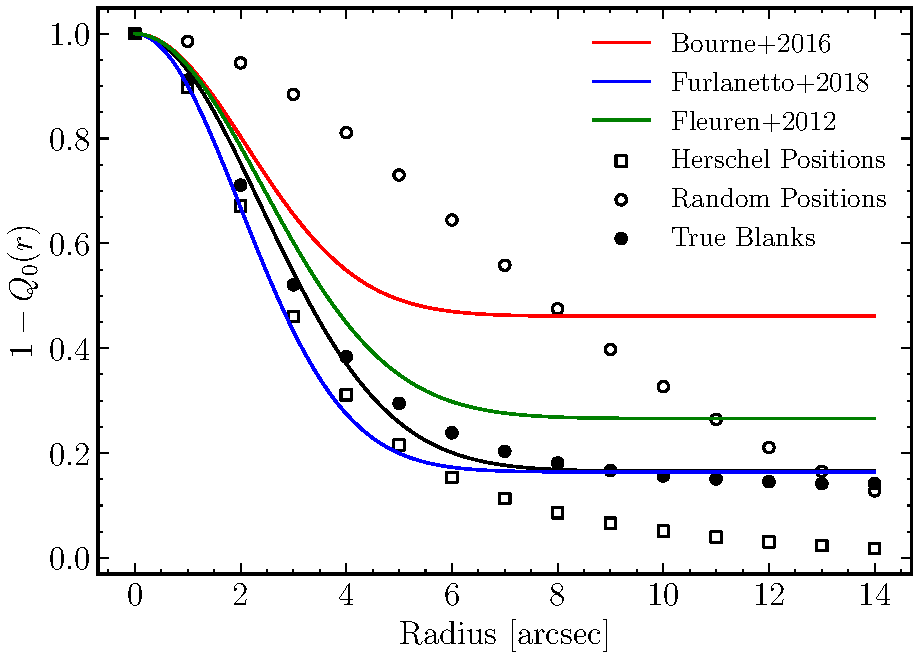
\includegraphics[width=\columnwidth]{Figures/Q_estimate.pdf}
	\caption{Estimates for the number of blanks (sources without VIKING candidates) as a function of the search radius, $r$. Open circles represent the number of blank random positions placed across the SGP, while open squares represent the number of blank SPIRE 250\,\micron positions from H-ATLAS. The filled circles shows the division of the former by the latter, representing our estimate for the true fraction of SPIRE sources that are blank on the VIKING images. The solid black line represents the best fit to the points using Equation \ref{eq:blanks_model}. The same model used in \citealt{Fleuren_2012}, \citealt{Bourne_2016} and \citealt{Furlanetto_2018} are shown as green, red and blue lines respectively.}
	\label{fig:Q_estimate}
\end{figure}

Previous estimates of $Q$ from r-band SDSS candidates in the other H-ATLAS fields have taken lower values as a result of the difference in depth between SDSS and VIKING. In DR1 \citealt{Bourne_2016} measured the value of $Q$ for all SDSS objects observed in the GAMA fields to be $0.539\pm0.001$, and \citealt{Furlanetto_2018} measured a near identical value of $Q=0.538\pm0.001$ in the NGP during DR2. However, my value of $Q$ is similar to that found by \citealt{Fleuren_2012}, $Q = 0.7342\pm0.0257$ and is almost identical to the value of $0.836\pm0.001$ found from the deep K-band analysis by \citealt{Furlanetto_2018}. As a collection, these estimates indicate that a survey of VIKING candidates returns a greater probability of observing a galaxy near a sub-mm source than an SDSS survey due to the increase in depth. A comparison between data releases due to the available input survey is made in Section [...]\todo[color=orange]{If a comparison between data releases is made, add the section reference here.} and in Table \ref{tab:data_release_input_surveys} I detail the various estimates made for $Q$ during analyses of H-ATLAS sources alongside their input surveys, passbands used and their depths.

\begin{table}
\centering
\begin{tabular}{|p{6.5cm}|p{3.5cm}|p{2.5cm}|p{4cm}|}
    \hline
    H-ATLAS & Input Survey & $Q$ Estimate & Reference \\
    \hline
    \hline
    Science Demonstration Phase (SDP) & SDSS -- ($r < 22.4$) & $0.583$ & \citealt{Smith_2011} \\ 
    Phase 1 GAMA9 & VIKING -- ($K_s < ??$) & $0.734\pm0.026$ & \citealt{Fleuren_2012} \\
    Data Release I & SDSS -- ($r < ??$) & $0.539\pm0.001$ & \citealt{Bourne_2016} \\
    Data Release II & SDSS -- ($r < ??$) & $0.538\pm0.001$ & \citealt{Furlanetto_2018} \\
    Data Release II & UKIRT -- ($K_s < ??$) & $0.836\pm0.001$ & \citealt{Furlanetto_2018} \\
    Data Release III & VIKING -- ($K_s < ??$) & $0.835\pm0.009$ & This work \\
    \hline
\end{tabular}
\caption{Comparison of the input survey passbands, depths and measured values of $Q$. From left to right the columns contain: i) the corresponding data release of H-ATLAS, ii) the input survey, passband used and its limiting magnitude, iii) the fraction of true sources observed on the survey images, $Q$, iv) reference.}
\label{tab:data_release_input_surveys}
\end{table}
\todo[color=orange]{Complete Table.}

\subsection{Positional Uncertainty of H-ATLAS Detections}

The fitting function of Equation \ref{eq:blanks_model} also provides an estimate for the standard positional error, $\sigma_{\textrm{pos}}$ which defines the width of the positional offset distribution $f(r)$. I measure this value to be $\sigma_{\textrm{pos}} = 2.388\pm0.065"$, representing the average error in the 250\,\micron positions. We see in Figure \ref{fig:Q_estimate} that $B(r)$ becomes flat at approximately 3$\sigma_{\textrm{pos}}$, suggesting that few counterparts are to be found at search radii greater than $\sim$ 7". It also interesting to note that the model underpredicts the number of blank sources between 4 $\lesssim$ r $\lesssim$ 8 arcsec, but overpredicts at the highest search radii. This has been observed previously (e.g. \citealt{Fleuren_2012}) and might suggest clustering of VIKING objects which is not modelled in $B(r)$.

The positional uncertainty has a dependency on the SNR of the sub-mm detection (\citealt{Bourne_2016}) and in theory should depend on the ratio between the FWHM of the observations and the SNR as given by

\begin{equation}
    \sigma_{\textrm{pos}} = 0.6\times\frac{\textrm{FWHM}}{\textrm{SNR}},
\label{eq:positional_uncertainty_theory}
\end{equation}

as detailed by \citealt{Ivison_2007} on the assumption of uncorrelated noise. However, the prefactor is likely to be increased by confusion noise in the maps and clustering (\citealt{Chapin_2011}; \citealt{Bourne_2014}) and so a scaling factor (typically about 1.09, corresponding to a redefined prefactor of $\sim$ 0.65) is applied and is more suitable for sources detected on sub-mm images. To define an individual value of the 1$\sigma$ positional uncertainty, and thus a separate $f(r)$ for each detection, I implement an empirical version of Equation \ref{eq:positional_uncertainty_theory} of the form

\begin{equation}
    \sigma_{\textrm{pos}} = k\times\frac{\textrm{FWHM}}{\textrm{SNR}},
\label{eq:positional_unceratinty_empirical}
\end{equation}

where $k$ is a constant to be determined. Using FWHM = 18", the fitted value of $\sigma_{\textrm{pos}} = 2.388$ and  the SNR of each 250\,\micron detection, I generate a set of $k$ values. I take the median value of the distribution of $k = 0.66$ as my constant. This value is used in Equation \ref{eq:positional_unceratinty_empirical} to determine $f(r)$ for each object's likelihood calculation.

A more refined method of determining $\sigma_{\textrm{pos}}$ is outlined in \citealt{Smith_2011} and applied in other works (e.g. \citealt{Bourne_2014}, \citealt{Bourne_2016} and \citealt{Furlanetto_2018}), though is also an empirical measurement. In such studies, a 2D histogram is derived for the offsets between sub-mm sources and optical/near-IR objects within a large box around each SPIRE source (typically 50" or more). This histogram can be modelled in shape by three contributing populations: i) a random background of chance alignments which should be observed as a constant since the probability of a chance alignment is equal along any line of sight; ii) the population of true IDs whose positional offset distribution follows $f(r)$ for a fraction $Q$ of all sources and iii) nearby counterparts that are physically correlated with the sub-mm source due to galaxy clustering but are not the true IDs, which requires an understanding of the cross-correlation between the sub-mm and optical/near-IR samples. Further details on the modelling of these histograms can be found in \citealt{Smith_2011}. By binning the sub-mm sources by their SNR and fitting the 2D histograms with a model considering the above contributions, an estimate can be made for $\sigma_{\textrm{pos}}$ as a function of SNR. Assuming a powerlaw dependence of the form $\sigma_{\textrm{pos}} = \sigma_{\textrm{pos}}(5) [\textrm{SNR}/5]^\alpha$ where $\sigma_{\textrm{pos}}(5)$ is the positional uncertainty of a 250\,\micron detection with SNR = 5, and by binning the sources further by sub-mm colour, it has been shown that the bluest SPIRE sources ($S_{250}/S_{350}$ > 2.4) have a dependence of $\sigma_{\textrm{pos}}$ on SNR that is not significantly different from the theoretical model given in Equation \ref{eq:positional_uncertainty_theory} (\citealt{Bourne_2016}; \citealt{Furlanetto_2018}). As shown in these studies the powerlaw function shifts to higher values of $\sigma_{\textrm{pos}}$ as we tend to redder sources. A possible explanation for a broader distribution of offsets for redder SPIRE sources is due to an increased probability of these sources being at higher redshifts and thus an increased contribution of foreground structures lensing the source. To avoid this bias, $\sigma_{\textrm{pos}}$ could be measured from the 2D histogram of positional offsets of the bluest sources, but for a model dependence that is reasonable for the majority of sources, a multiplicative factor should be included, leading to the prefactor of $k$ commonly assumed being larger than 0.6. Given that the simple method used here provides a similar value of $k$, I do not expect there to be any systematic differences in the likelihood calculations for SGP sources and the aforementioned papers as a result of the different methods used to calculate $\sigma_{\textrm{pos}}$.

\section{Likelihood Ratio Results}

I apply the likelihood ratio to all possible VIKING counterparts within 15" of a SPIRE source. The catalogue contains 193,527 sub-mm sources, of which 190,788 have at least one possible counterpart identified within the search radius. Within this sample, 180,030 are sources with SNR$_{250}$ > 4. Having identified each source with its highest reliability counterpart I find that 181,373 (95.1\%) are sources with VIKING identifications indicating the source is a galaxy and 9,415 (4.9\%) with stellar classifications. 

In keeping with previous studies I define reliable matches as those sources with counterparts having $R \geq 0.8$ in order to minimize the number of false counterparts while maintaining a sample that is dominated by sources with a low chance of blending and thus the FIR emission is likely dominated by a single source. I identified 111,065 reliable near-IR counterparts, representing 58.2\% of all sources with at least one possible candidate. Of the reliable IDs, 110,374 (99.4\%) are classified as extragalactic and 691 (0.6\%) as stellar. The increase in the fraction of galaxies and reduction in stars compared to the input VIKING survey suggests that the LR method is highly biased against stars as is intended.

On the assumption that a source that is erroneously matched with a counterpart has a probability of $1 - R$, we can estimate the false ID rate for our reliable matches:

\begin{equation}
    N_{\textrm{False}} = \sum_{R_i \geq 0.8} (1 - R_i) = 5,343.
\label{eq:false_ids}
\end{equation}

I predict that there are 5,343 "false reliable" IDs in the SGP, representing 4.8\% of the reliable sample. This can be compared to values of 4.7\% in the GAMA fields and the NGP (optical SDSS matching), 4.5\% for the NGP (near-IR deep matching) and 4.2\% during the SDP. While the value for the SGP is in keeping with the other H-ATLAS fields, it is the highest false identification rate. It would be expected that the near-IR analyses would have the lowest false identification rates as the optical r-band restricts the limiting redshift of the counterparts to lower redshifts than the near-IR K-band (see Figure [...]\todo[color=orange]{If a figure showing the different redshift depths of surveys is made, add reference here}). As a result, the contamination of high redshift sub-mm sources that are falsely identified with low redshift optical counterparts is expected to be higher, increasing the false identification rate. However, in the analysis of the SGP, we choose to use an increased search radius of 15" (compared to 10" as used in previous H-ATLAS studies) which increases the average number of counterparts found per source. Given the requirement of the LR method that the sum of the reliabilities of all possible candidates to a source must not exceed one, the increased average number of candidates reduces the average reliability of the true ID and thus increases the false identification rate - likely by a factor greater than the reduction caused by using the near-IR VIKING survey compared to SDSS. Further discussion on the effect of increasing the search radius is made in Section X [...]\todo[color=green]{Add reference to multiplicity section}. The initial choice to use a search radius of 15" came from recent studies suggesting that genuine associations are found on the VIKING images beyond 10" as a result of gravitational lensing (\citealt{Bakx_2020}). In the final SGP \textit{Herschel}+VIKING catalogue, we wish to keep such VIKING objects despite them being highly unlikely to have significant reliability values.

The completeness, $\eta$, of the reliable sample is defined as the fraction of 250\,\micron sources that are recovered with a reliability greater than 0.8 (\citealt{Smith_2011}) and can be estimated as

\begin{equation}
    \eta = \frac{n(R \geq 0.8)}{n(\textrm{SNR}_{250} \geq 4) \times Q},
\label{eq:completeness}
\end{equation}

where the numerator is the size of the reliable sample and the denominator estimates the true number of sources. As would be expected, a value of unity for $\eta$ would imply that the fraction of all counterparts deemed reliable has reached its theoretical maximum, $Q$. Another important diagnostic is the cleanness, $C$, of the reliable ID sample, an estimate for the number of sources that are not spurious matches, given by

\begin{equation}
    C = 1 - \frac{N_{\textrm{False}}}{N_{\textrm{250\,\micron}}}.
\label{eq:cleanness}
\end{equation}

At a reliability cut of 0.8, I find that the completeness of the extragalactic reliable sample is $\eta$ = 78\%, which is similar to the completeness values found for the NGP and GAMA fields of 74\% and 73\% respectively. In Figure \ref{fig:completeness_and_cleanness} I illustrate how the completeness and cleanness change over a range of different reliability thresholds. We see that a cut at $R \geq 0.8$ selects a highly clean sample at the expense of completeness. While an increase in the reliability cut would yield a marginally cleaner sample, it would be offset drastically by a fall in completeness. A decrease in the choice of minimum reliability would lead to an increase in completeness at little expense of the cleanness, but to maximize the completeness would be to set a reliability so low that a one-to-one matching between sub-mm sources and counterparts would not be a guarantee. At $R \geq 0.8$ we set a boundary for which there is a good compromise between the two diagnostic parameters.

\begin{figure}
    \centering
	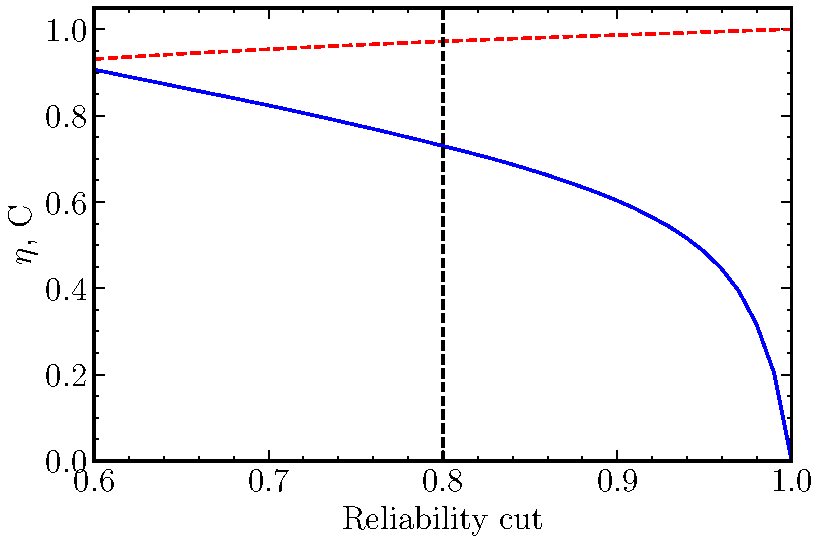
\includegraphics[width=\columnwidth]{Figures/completeness_and_cleanness.pdf}
	\caption{The completeness, $\eta$, and cleanness, C, of the SGP sample as a function of various minimum cuts in reliability, illustrated as solid blue and red dashed lines respectively. The vertical dashed line reprents the reliability cut used in all H-ATLAS fields (R $\geq$ 0.8).}
	\label{fig:completeness_and_cleanness}
\end{figure}

\section{Properties of \textit{Herschel} Sources and their Counterparts}

In the subsequent sections I report on the bulk properties of the SMGs in the SGP field that can be obtained from a combination of the sub-mm and near-IR data. While the far-IR to sub-mm wavebands unveil the dusty, cold regions of the Universe, the inclusion of the near-IR data (the $K_s$-band covers wavelengths between $\sim$ 2--2.3\,\micron) samples the peak of the emission of older stars and as such is suited for examining the stellar properties of a galaxy such as its stellar mass as it traces the total stellar content of a galaxy (\citealt{Cole_2001}; \citealt{Bell_2003}). Moreover, at high redshifts (z $\gtrsim$ 0.5) the rest frame optical bands are observed in the near-IR, meaning that the VIKING counterparts at higher redshifts also probe young stellar populations.

\subsection{Submillimeter Colours}
% Include a comparison of sub-mm colours across the data releases
\subsection{Near-IR Properties of \textit{Herschel} Sources}
% Include a comparison of magnitude distributions

\subsection{Multiplicity of Counterparts}
One important disadvantage to using the LR method to identify multiwavelength counterparts to low resolution sources is that it assumes a one-to-one matching of sources and counterparts. Given that we are restricted to a user defined reliability threshold for our sample, and that the sum of reliabilities for all possible candidates to a source may not exceed one, our reliable sample becomes biased against multiple systems, such as merging galaxies, members of a cluster or non-physical associations such as confusion due to blending, as their combined reliabilities reduces the maximum reliability of the chosen ID. For example, consider two galaxies that form part of a cluster that are observed with VIKING close to a SPIRE source. It is reasonable to imagine that these two sources may have similar K-band magnitude and radial offset from the source, and particularly if they are close to the sub-mm emission, may both have high likelihoods. In such a case, either source may be considered the true ID to the source (and in reality both are likely associated), but the use of Equation \ref{eq:reliability_multiple_counterparts} to define their reliabilities leads to the following simplification (assuming the likelihoods are much larger than $1-Q$):

\begin{equation}
    R_j \sim \frac{L_j}{\sum_i L_i} \sim \frac{L_j}{2L_j} \sim 0.5.
\end{equation}

In this scenario, neither counterpart would be considered the true ID and thus we are biased against multiple systems. 

In Table \ref{tab:multiplicity} I show the number of SPIRE sources and the fraction of those with reliable counterparts as a function of the number of possible candidates observed within 15". We observe that the fraction of sources with reliable counterparts decreases with increasing multiplicity. This suggests that the sample is in part incomplete because we miss sources where there is more than one genuine counterpart. In Figure \ref{fig:multiplicity} I show the reliable fraction of sources as a function of multiplicity for the SGP compared with previous H-ATLAS data releases in other fields. Comparing to the Science Demonstration Phase (\citealt{Fleuren_2012}), GAMA (\citealt{Bourne_2016}) and the NGP (\citealt{Furlanetto_2018}), we see that reliability fraction declines more slowly, peaks at slightly higher average $N_{\textrm{Match}}$ and is lower for sources where there is only a single possible counterpart. These effects are most likely a result of the increased search radius of 15" used during the SGP analysis compared to 10" in the other fields, which per source equates to a 2.5 factor increase in the search area ($A_{\textrm{SGP}}/A_{\textrm{Other}} = \pi r_{\textrm{SGP}}^2/\pi r_{\textrm{Other}}^2 = 225\pi/100\pi = 2.5$). The increased $r$ means that we are more likely to observe a reliable counterpart, but also means we increase the probability of matching erroneously to a background source, which would explain why we observe a higher false identification rate for the reliable sample of the SGP. The low fraction of reliably matched sources at $N_{\textrm{Match}} = 1$ may be due to an increase in unassociated VIKING objects being selected as the true ID. Occassionally, the chosen ID will be unassociated with the sub-mm source, but selected solely for being the only possible candidate despite having a large radial offset. This effect is more pronounced for an increase in $r$. In Table \ref{tab:multiplicity} we see that the average offset between VIKING galaxy and source is substantially higher when the galaxy is the only possible candidate, suggesting that some fraction of these sources are erroneously matched. However, the shift of the peak to higher $N_{\textrm{Match}}$ is likely due to the greater ability to discern between true IDs and chance alignments when the same number of candidates are spread over a larger surface area. Another reason why the reliable fraction is so low for $N_{\textrm{Match}} = 1$ is that a large fraction of the stellar candidates will fall in this bin as stars tend to be isolated (\citealt{Bourne_2016}) and therefore reduce the average reliability of these sources. Lastly, the increase in the search area around each SPIRE source means that the fraction of reliably matched sources does not fall until much higher $N_{\textrm{Match}}$, leading to a flatter distribution.


\begin{table}
    \centering
    \begin{tabular}{|p{2.5cm}|p{2.5cm}|p{2.5cm}|p{2.5cm}|p{4cm}|}
        \hline
        $N_{\textrm{Match}}$ & $N_{\textrm{SPIRE}}$ & $N_{\textrm{Reliable}}$ & Percent & Av. Separation [arcsec] \\
        \hline
        \hline
        0 & 2,739 & 0 & 0 & 0 \\
        1 & 11,692 & 5,477 & 47 & 6.3 \\
        2 & 24,268 & 14,568 & 60 & 4.7 \\
        3 & 32,948 & 20,396 & 62 & 4.1 \\
        4 & 33,526 & 20,383 & 61 & 3.8 \\
        5 & 27,745 & 16,359 & 59 & 3.6 \\
        6 & 20,236 & 11,563 & 57 & 3.4 \\
        7 & 12,999 & 7,155 & 55 & 3.4 \\
        8 & 8,079 & 4,355 & 54 & 3.3 \\
        9 & 4,983 & 2,640 & 53 & 3.4 \\
        10 & 3,017 & 1,643 & 54 & 3.3 \\
        \hline
    \end{tabular}
    \caption{The reliable fraction illustrated as a function of the number of candidates observed per source. From left to right the columns contain: the number of possible candidates per source; the number of SPIRE sources that have the number of candidates specified in column one; the number of those sources whose best counterpart has a reliability greater than 0.8; the reliable fraction given as a percentage; and the average separation between the chosen ID and the source in arcsec.}
    \label{tab:multiplicity}
\end{table}

\begin{figure}
    \centering
    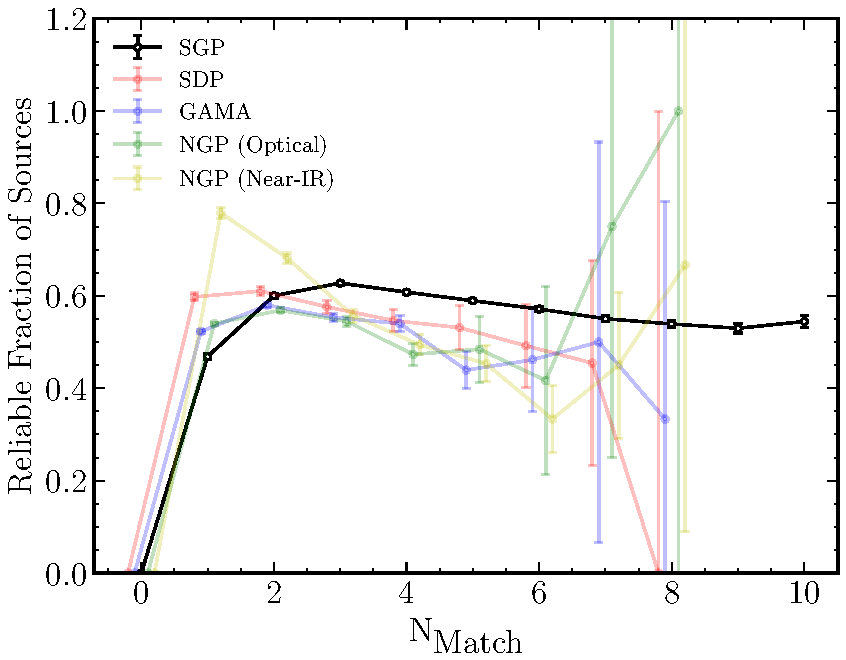
\includegraphics[width=\columnwidth]{Figures/multiplicity.pdf}
    \caption{The fraction of \textit{Herschel} sources with reliably matched counterparts as a function of the number of observed candidates. The results from various H-ATLAS fields are shown as the following lines: SGP (black, this work); SDP (red, \citealt{Smith_2011}); Phase 1 GAMA9 Field (blue, \citealt{Fleuren_2012}), GAMA (green, \citealt{Bourne_2016}), NGP (optical in yellow, near-IR in pink, \citealt{Furlanetto_2018}). All other works used a maximum search radius of 10" while the SGP analysis used 15". For clarity each line has been offset in $N_{\textrm{Match}}$ by a different value.}
    \label{fig:multiplicity}
\end{figure}

We can estimate the number of sources that have multiple genuine associations that were missed by the LR method by assuming that all candidates are associated with a single source if their combined reliabilities is greater than 0.8, but are missed because no individual counterpart meets the threshold. I find [...]\todo[color=orange]{Do calculation} such sources, however, due to the increased maximum $r$ and consequently increased average number of candidates per source, even moderately valued $R$ counterparts combine to exceed the reliability cut. Alternatively, we could use the likelihood values, $L$, for each counterpart, rather than their reliability as the likelihood has no upper limit unlike the bounds on reliability, $R \in [0, 1]$. From Equation \ref{eq:reliability_multiple_counterparts} a reliability of 0.8 or greater corresponds to $L > 0.66$, assuming a single candidate and a value of $Q = 0.835$. An estimate for the number of lost sources with multiple associated counterparts can be made assuming that a source with a best matched counterpart with $L > 0.66$ but $R < 0.8$ is influenced by nearby candidates. I find 33,967 sources that satisfy these conditions. However, this is likely an overestimate of the true number as a large fraction of these IDs will be due to a mixture of true mergers or close groups and chance alignments; a measure for the probability that two or more counterparts are physically associated is required to potentially identify galaxy groups or mergers.

An improved estimate that removes chance alignments can be made considering the photometric redshifts of the VIKING objects (the method of obtaining photometric redshifts for the VIKING sample is presented in Section \ref{sec:phot_z_VIKING}). As shown in \citealt{Fleuren_2012}, chance matches along the line of sight can be ruled out by comparing the redshifts of all possible matches, and considering them to be associated if they fall within $\sim$ 10\% of each other for photometric redshifts or $\sim$ 5\% if using spectroscopic redshifts. While this is a simple and effective method, it does not rule out sources that happen to lie on a similar line of sight to unrelated groups or mergers of galaxies (and the true ID remaining unmatched or beyond the VIKING survey limit). In the following, I describe a new method in which we use the background distribution of VIKING sources (as used for estimating the magnitude distribution of true counterparts in Section \ref{sec:true_counterparts_distribution}) to estimate the probability that a pair of VIKING galaxies with similar redshifts are associated with the sub-mm source. 

Firstly, I restrict both the SGP and background catalogues to contain only sources with two or more counterparts and I restrict this further to counterparts found within 8", as this is where the majority of $L > 0.66$ counterparts are found, reducing the chance of selecting pairs of galaxies that are unrelated to the source. For each position in both catalogues, I identify the pair of galaxies with the closest redshifts and calculate the difference in their redshifts divided by the error in the difference, i.e. $\Delta z/\sigma_{\Delta z}$. In Figure \ref{fig:delta_z_multiplicity} I show the probability distribution functions (PDFs) of $\Delta z/\sigma_{\Delta z}$ for the SGP catalogue (red line) and the background catalogue (black line). When a background subtraction of the SGP catalogue is made, we observe an excess close to $\Delta z = 0$ (blue line) where the area of this peak represents the probability that a close pair of VIKING galaxies is indeed related to the SPIRE source. I fit a Gaussian profile to the excess and calculate this probability to be 2 -- 5\% depending on the size of the bins used to generate the PDFs. By multiplying this probability by the total number of SPIRE sources for which we observe a close pair of VIKING galaxies, in this case we take this to be the width of the peak, $-0.1 \lesssim \Delta z/\sigma_{\Delta z} \lesssim 0.1$, I find an estimate for the number of \textit{Herschel} sources with genuine multiple counterparts of $\sim$ 400 -- 1,000.

\begin{figure}
    \centering
    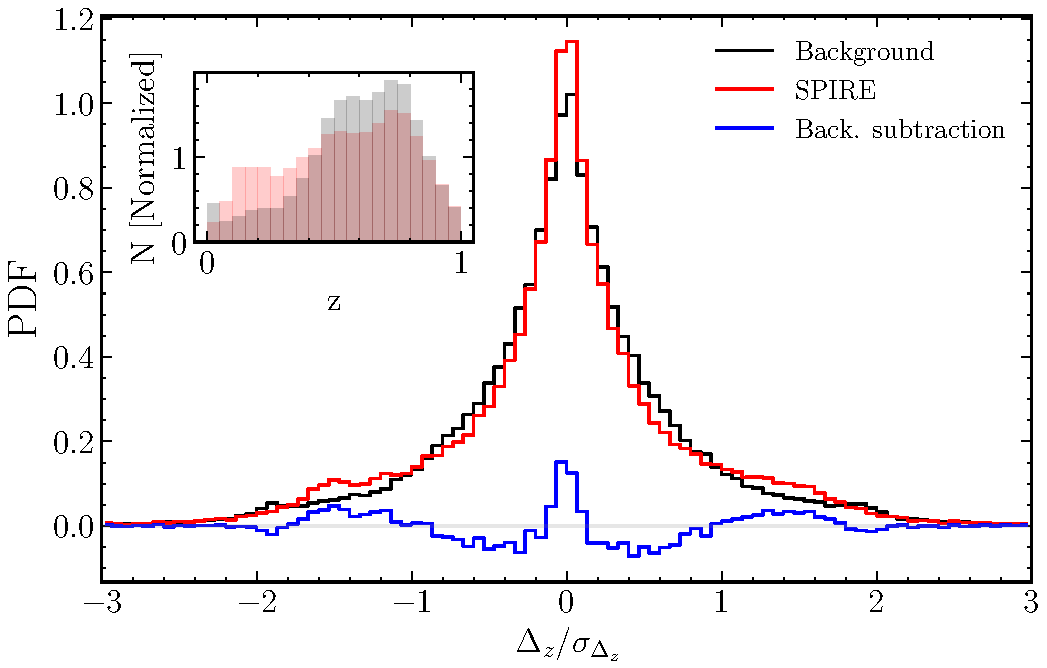
\includegraphics[width=\columnwidth]{Figures/delta_z_multiplicity.pdf}
    \caption{Probability distribution functions of $\Delta z/\sigma_{\Delta z}$, the difference between photometric redshifts of VIKING counterparts divided by the error in their difference, for pairs of galaxies located near 250\,\micron positions (within 8") in the SGP catalogue (red histogram) and near randomly located positions (black histogram). The blue histogram represents a background subtraction of the former. The excess located at $\Delta z = 0$ represents the subset of VIKING galaxy pairs with similar redshifts that are associated with the SPIRE source. The inset figure shows the normalized redshift distribution of VIKING counterparts observed within 8" of 250\,\micron positions in red and random positions in grey.}
    \label{fig:delta_z_multiplicity}
\end{figure}

It should be noted that this method is independent of the LR method and the resulting reliability values, and so the pair of VIKING objects chosen for each source does not always contain the candidate with the highest reliability. In total there are 70,880 sources where we observe two or more candidates with estimated photometric redshifts (within 8" of the source), of which approximately three quarters have best counterparts that are also part of the "redshift pair". The selected pairs for the remaining quarter of sources may be the locations of unassociated galaxy interactions or multiple systems related to the sub-mm source that is overlooked by the one-to-one matching of the LR method. The subset used here is approximately one third of all sources in the SGP (70,880/193,527) and so we expect mant more galaxy interactions and groups to be in the full SGP catalogue. We also note that the fraction accounting for all sources may be higher as there is evidence to suggest that the merger rate of galaxies evolves with redshift and reaches a peak at $z \sim 1.2$ (e.g. \citealt{Bell_2006}; \citealt{Ryan_2008}). If this is true, then a large fraction of interacting systems may be those beyond the VIKING detection limit and therefore lie in the blank SPIRE fields.

\subsection{Photometric Redshifts of Submillimeter Sources}
\label{sec:phot_z_Herschel}

Any study on the evolution of fundamental properties of extragalactic sources requires an estimate for the age of the galaxy and therefore its redshift. Having crossmatched the sources detected on the sub-mm images with the sources on the VIKING images, we can begin to construct spectral energy distributions (SEDs) that places constraints on the stellar properties as well as the dust emission. 

The dust emission can be well approximated using a two-temperature modified blackbody model (see Section [...]\todo[color=green]{Add reference to blackbody functions when written} for a more detailed description on modified blackbody functions). A characteristic SED that can be used to approximate the SED of a typical H-ATLAS source is presented in \citealt{Pearson_2013} and takes the form:

\begin{equation}
    S_\nu = A[B_\nu(T_{\textrm{hot}})\nu^\beta + \alpha B_\nu(T_{\textrm{cold}})\nu^\beta],
\label{eq:pearson_sed_model}
\end{equation}

where $S_\nu$ is the flux density of the source at the rest frame frequency, $\nu$, $A$ is a normalization factor, $B(T)$ represents the Planck function at temperature $T$, of which we assume two dust temperatures, $T_{\textrm{hot}}$ and $T_{\textrm{cold}}$, $\beta$ is the dust emissivity index and $\alpha$ represents the fraction of cold dust mass to hot dust mass. Using a sample of 40 H-ATLAS sources with spectroscopic redshifts, the optimal set of parameters were measured to be $T_{\textrm{hot}} = 46.9$\,K, $T_{\textrm{cold}} = 23.9$\,K and $\alpha = 30.1$ (assuming a fixed $\beta = 2$). This leaves a model with only two free parameters, the normalization and the redshift; a necessary simplification given that each source had at most three flux densities at the central wavelengths of the SPIRE bands (the PACS 100 and 160\,\micron flux densities were not included as the \textit{Herschel} images are less sensitive at these wavelengths). For each source the normalization and redshift were varied until a minimum chi squared was reached:

\begin{equation}
    \chi^2 = \sum_i \frac{S_i - S_{i,m}}{E_i^2},
\end{equation}

where $S_i$ is the flux density at each SPIRE wavelength, $i$, $S_{i,m}$ is the model prediction of the flux and $E_i$ is the error on the flux at wavelength $i$. 

While all sources in the SGP have estimates for their flux and flux errors at the SPIRE wavelengths in the second data release, the errors do not account for calibration errors. The calibration error is formed of two parts: i) the main contribution comes from uncertainty in the models used for calibration objects, which in the case of SPIRE is Neptune and for PACS is a group of stars and asteroids. This error is correlated between the bands and is approximately 4\% for SPIRE; ii) a contribution uncorrelated between bands of 1.5\% (\citealt{Valiante_2016}). While the correlated error scales all fluxes by the same amount, and therefore does not impact on the $\chi^2$, the uncorrelated errors do contribute and are calculated by adding in quadrature the errors in the catalogue with the errors obtained by multiplying the flux density of each source by 1.5\% such that $E_i = \sqrt{\sigma_{S_i}^2 + (S_i \times 0.015)^2}$, where $S_i$ and $\sigma_{S_i}$ are the flux and flux density of each source at wavelength $i$ from the DR2 catalogue presented in \citealt{Valiante_2016} and \citealt{Maddox_2018}.

The upper and lower 1$\sigma$ errors on our photometric redshifts were taken at the redshifts above and below the best-fitting value at which the $\chi^2$ increases by 1. When taking all sources collectively, the mean reduced chi-squared ($\chi_\nu^2 = \chi^2/\nu$ where $\nu$ is the number of degrees of freedom) should have a value of $\sim$ 1 if the model sufficiently represents the data. A mean value of $\chi_\nu^2 > 1$ would suggest that the model is not a good representation of the data while a mean value $\chi_\nu^2 < 1$ implies that either the model has too many free parameters or that the errors on the data are too large. The $\chi^2$-minimization technique applied to the sources in the SGP yields a mean value for $\chi_\nu^2$ of 0.55. Given that the model requires only two free parameters, it is more likely that this low value is a result of overestimated flux uncertainties than the two-temperature blackbody model being an unrepresentative model for the H-ATLAS sources. The resulting errors on the photometric redshifts account for all relevant uncertainties in the flux densities, but does not account for uncertainty in the model SED of \citealt{Pearson_2013}, given that high-redshift \textit{Herschel} galaxies have been shown to have a variety of SED shapes (\citealt{Bakx_2018}). The H-ATLAS sources used to generate the characteristic SED are intrinsically bright (facilitating their spectroscopic redshift search) and thus have fractionally smaller errors on their flux densities than the full H-ATLAS sample. This results in errors in the photometric redshifts smaller than appropriate for the variety of sources observed in H-ATLAS. For this reason, the redshift error estimated by \citealt{Pearson_2013}, $\Delta z/(1+z) = 0.12$, represents a fundamental redshift error that is caused by the diversity of real galaxy SEDs and should be taken as a minimum redshift error. For $\sim$ 9\% of sources the estimated redshift error is lower than this minimum value and we have therefore replaced the redshift error from the SED fitting with this minimum error. The median redshift of the sub-mm sources in the SGP is $\sim$ 1.4 and has a peak at a similar value. The distribution of photometric redshifts extends to very high $z$; it is predicted that more than $\sim$ 100 sub-mm sources in the SGP lie at redshifts greater than 5. The redshift distribution of \textit{Herschel} sources from the third data release can be seen in Figure \ref{fig:redshift_distribution}.

\subsection{Photometric Redshifts of VIKING Counterparts}
\label{sec:phot_z_VIKING}

I obtain photometric redshifts for the VIKING counterparts by matching the catalogue to the SGP data within the \textit{Herschel} Extragalactic Legacy Project (HELP; \citealt{Vaccari_2016}; \citealt{Shirley_2019}). HELP provides an extensive catalogue of extragalactic sources observed with \textit{Herschel} over a number of fields and provides overviews of optical and near-IR surveys that are available within these fields. The method used to produce the photometric redshifts catalogued within HELP is based on the template-fitting method of \citealt{Duncan_2018a} and includes further estimates using a machine learning technique as presented in \citealt{Duncan_2018b}.

The approach combines template fitted redshifts with machine learning redshifts to create a Bayesian combination of estimates. Three different sets of templates were used: the default library of SEDs provided with the photometric redshift code \texttt{EAZY} (\citealt{Brammer_2008}); the XMM-COSMOS templates of \citealt{Salvato_2009} and \citealt{Salvato_2011}, which cover a wide range of galaxy spectral types as well as active galactic nuclei (AGN) and quasi-stellar object (QSO) templates; and the Atlas of galaxy SEDs presented in \citealt{Brown_2014}, a set of 129 galaxy SED templates based on a range of nearby galaxies including ellipticals, spirals and luminous IR galaxies (starbursts and AGN). These three sets of templates were chosen for their common use in the literature and their coverage of the range of colours observed in local galaxies. To generate the set of photometric redshifts from machine learning, a training set is compiled from a sample of 48,995 galaxies with spectroscopic redshifts in the SGP plus additional redshifts from the three GAMA fields (the surveys used in the training set include the 2dF, 6dF, 2MRS and SRSS2 surveys). Three separate redshift estimates were made using three sets of filters: $u$, $g$, $r$ and $i$ from OmegaCAM on the VLT Survey Telescope; $g$, $r$, $i$, $z$ and $y$ from the Dark Energy Camera (DECam) on the Victor M. Blanco 4-meter Telescope; and $J$ and $K_s$ from the VISTA InfraRed CAMera (VIRCAM) on VISTA (along with the aforementioned $g$, $r$ and $i$ bands from OmegaCam). The machine learning redshifts were generated using the redshift code GPz (\citealt{Almosallam_2016}). The full posterior distributions of all template and machine learning redshift estimates for each source in HELP were then combined using the Hierarchical Bayesian combination method described in \citealt{Dahlen_2013}.

The method used by HELP described above provides the full photometric redshift posterior distribution for each identified source. The assumed redshift of each object is taken from the posterior distribution in the following way. First, an 80\% highest probability density (HPD) credible interval (CI) was calculated by starting at the peak redshift probability and lowering a threshold until 80\% of the total probability is above the threshold. The resulting HPD CI may have two or more peaks, in such cases they are ranked from the most to least probable based on their peak value. I used the median redshift of the primary peak as the photometric redshift of each source. To estimate the redshift errors, I assumed that the upper and lower boundaries of the HPD CI defines a Gaussian in the posterior distribution, symmetric about some mean redshift value. I then transform the 80\% credible interval into 1$\sigma$ errors assuming a Gaussian distribution where an 80\% CI is equal to 1.282$\sigma$.

In total there are 29,790,690 objects with photometric redshifts in the SGP catalogue of HELP. I use a 0.5" matching radius to find the nearest neighbour to all the VIKING counterparts in the H-ATLAS field. This yields 542,302 (54\%) redshifts, corresponding to 82,195 sources in the reliable ID sample (74\% of the reliable sample). Given the limiting magnitude of the VIKING survey the majority of the near-IR counterparts have redshifts < 1. This naturally represents only a fraction of all H-ATLAS sources as they extend to redshifts as high as $\sim$ 5 -- 6, but is an improvement on the depth of galaxies matched to the SDSS survey which loses its high levels of completeness beyond z $\sim$ 0.4. The distribution of photometric redshifts of the VIKING counterparts can be seen in Figure \ref{fig:redshift_distribution}. The typical uncertainty on the redshifts is smaller for the counterparts ($\sigma_z \sim 0.21$) than it is for the sub-mm sources ($\sigma_z \sim 0.51$), thus to create a redshift distribution in which we have one redshift per source, I preferentially chose to use the redshift of the near-IR counterpart if avilable, otherwise I would use the estimate made from the sub-mm fluxes.

\begin{figure}
    \centering
    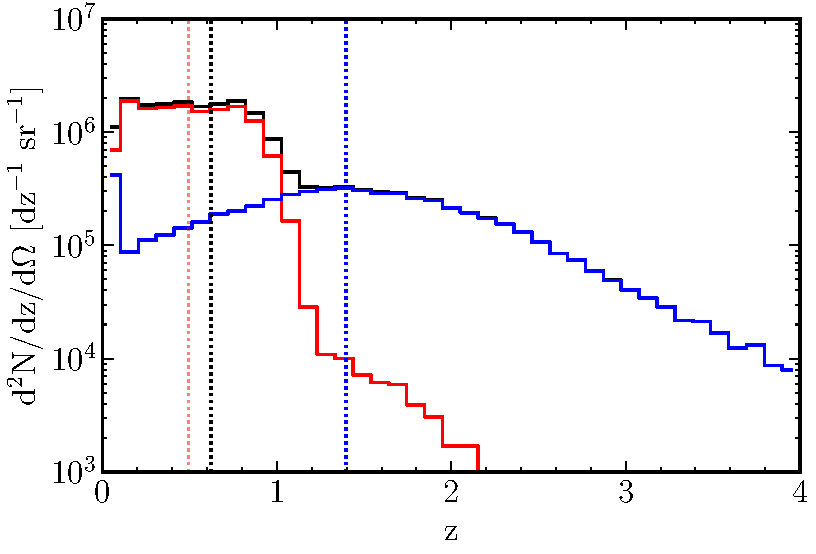
\includegraphics[width=\columnwidth]{Figures/redshift_distribution.pdf}
    \caption{Photometric redshift distribution of the sources in the SGP field of H-ATLAS. The blue line represents the distribution of redshifts obtained from the SED fitting of the SPIRE fluxes to each sub-mm source; the red line represents the distribution of redshifts for the near-infrared counterparts observed in VIKING, as matched with the \textit{Herschel} Extragalactic Legacy Project, and the black line represents the distribution of the best redshifts for all sources, preferentially selecting the redshift of the counterpart. The median redshifts are $z_{\textrm{sub-mm}} = 1.40$, $z_{\textrm{near-IR}} = 0.49$ and $z_{\textrm{best}} = 0.62$ and are illustrated by the dotted red, blue and black vertical lines respectively.}
    \label{fig:redshift_distribution}
\end{figure}

\section{Gravitational Lensing in the SGP}

When the light from a distant galaxy is close to the same line of sight as a foreground mass, whether that be an individual galaxy (likely a massive elliptical) or galaxy cluster, the magnification of the background source due to the deflection of the light makes the galaxy appear brighter with a larger angular size. This gravitational lensing makes these systems ideal targets for studying intrinsically faint and distant galaxies that may otherwise be impossible to probe. This effect can be exploited to generate prime targets for studies of the physical conditions in distant star forming galaxies at resolutions otherwise unattainable and also provide potential as subjects for studies of the cosmological parameters (e.g. \citealt{Kochanek_1992}; \citealt{Kochanek_1996}; \citealt{Grillo_2008}; \citealt{Oguri_2012}; \citealt{Eales_2015}) and the evolution of the equation of state of dark matter (e.g. \citealt{Zhang_2009}). 

However, identifying large samples of lenses can be time-consuming while searches are made through large surveys and imaging to find signs of gravitational lensing (e.g. Einstein rings). Moreover, if a blind search for lensing events were made it would require large areas to be surveyed due to their rarity. However, blank field sub-mm surveys have been shown to contain a vast number of lensing events when considering the brightest sources on sub-mm images (e.g. \citealt{Blain_1996}; \citealt{Perrotta_2002}; \citealt{Negrello_2007}; \citealt{Paciga_2009}; \citealt{Bakx_2020}). We note that the occurence of gravitational lensing events can be high in the sub-mm because of the high average redshift (z $\gtrsim$ 1) of sub-mm selected galaxies. The brightest sources (typically selected using a flux cut of $S_{\textrm{500\,\micron}} \gtrsim$ 100\,mJy) that populate the bright tail of the sub-mm counts contain several populations. These include low redshift (z $\lesssim$ 0.1) spiral and starburst galaxies, higher redshift AGNs and candidates for lensed sources. Given that the former populations can be easily identified and removed from shallow optical and radio surveys, a flux-limited sample of sub-mm sources can provide a sample of candidate lensing systems with low contamination using a straightforward selection process. This method has been used extensively in previous studies of \textit{Herschel} surveys; \citealt{Negrello_2010} produced the first sample of strongly lensed \textit{Herschel} galaxies (SLGs), presenting 5 lensed galaxies within the SDP, \citealt{Wardlow_2013} identified 11 lensed galaxies from the 95\,deg$^{2}$ area of the \textit{Herschel} Multi-tiered Extragalactic Survey (HerMES; \citealt{Oliver_2012}). Subsequently, \citealt{Nayyeri_2016} presented a further 77 candidates from the 372\,deg$^{2}$ of sky covered by the HerMES Large Mode Survey (HeLMS) and the \textit{Herschel} Stripe 82 Survey (HerS; \citealt{Viero_2014}). More recently, \citealt{Negrello_2017} identified a sample of 80 candidates for lensing from $\sim$ 600\,deg$^{2}$ of the H-ATLAS. In the subsequent sections I shall present a statistical sample of candidate lensed sources from the SGP, first by selecting the brightest sources using the method outlined in \citealt{Negrello_2017}, then extending this to lower flux densities by estimating the likelihood of gravitational lensing based on the redshift distributions of the sub-mm sources and their near-IR counterparts.

\subsection{The Brightest Lensed Sources}

The number counts of unlensed sources falls rapidly at 500\,\micron flux densities above $\sim$ 100\,mJy because of the steep luminosity function. For a given luminosity, the probability of a galaxy having an intrinsic brightness of such high flux density becomes much lower than the probability that an intrinsically fainter source is magnified due to gravitational lensing. Therefore, the first step is to select all sources with $S_{\textrm{500\,\micron}}$ > 100\,mJy. This first selection resulted in 179 sources, 175 of which had at least one VIKING counterpart associated. 

\begin{table}
    \centering
    \begin{tabular}{|p{5cm}|p{3.5cm}|p{2.5cm}|p{2.5cm}|p{2.5cm}|}
        \hline
        H-ATLAS IAU Name & NED Identification & $S_{\textrm{250\,\micron}}$ [mJy] & $S_{\textrm{350\,\micron}}$ [mJy] & $S_{\textrm{500\,\micron}}$ [mJy] \\
        \hline
        \hline
        HATLASJ014310.0-320056 & PKS 0140-322 & 96.0$\pm$7.5 & 119.5$\pm$8.4 & 122.4$\pm$9.0 \\
        HATLASJ014503.4-273333 & [HB89] 0142-278 & 131.4$\pm$7.8 & 179.2$\pm$8.8 & 234.4$\pm$9.0 \\
        HATLASJ222321.6-313701 & PKS 2220-318 & 86.0$\pm$9.5 & 110.9$\pm$10.5 & 131.9$\pm$11.7 \\
        HATLASJ224838.6-323551 & [HB89] 2245-328 & 119.2$\pm$7.7 & 152.8$\pm$8.3 & 194.7$\pm$8.6 \\
        HATLASJ235347.4-303746 & PKS 2351-309 & 77.1$\pm$7.4 & 96.6$\pm$8.4 & 103.1$\pm$8.9 \\
        \hline
    \end{tabular}
    \caption{The blazars with 500\,\micron flux density > 100\,mJy identified in the SGP using NED.}
    \label{tab:blazars}
\end{table}

The low-redshift spirals and flat spectrum radio galaxies that contaminate this sample were identified and removed by searching the location of the sources with the NASA/IPAC Extragalactic Database (NED). I also removed two variable stars (HATLASJ012658.0-323234 -- R Sculptoris and HATLASJ225519.6-293644 -- V Piscis Austrini) and five blazars, as listed in Table \ref{tab:blazars}. In total 131 local galaxies were clearly identified from their resolved imaging in NED. These objects have much "bluer" sub-mm colours than the remaining sample, suggesting that despite their equally high flux density they are separate populations at different redshifts. The remaining 41 sources with "redder" sub-mm colours and thus most likely to be at high redshifts, I retained as the list of candidate lensed sources in the SGP. The complete sample of sources is tabulated in Appendix \ref{app:candidate_lenses_bright}.

\subsection{Extending the Search for Lenses to Lower Fluxes}

\section{The Full \textit{Herschel}-ATLAS}
% Include correlations with redshift now they have been described (e.g. flux and magnitude against redshift)
% Include a description of the full H-ATLAS: a legacy product that has no plans for being replaced

\section{Conclusions}

\listoftodos